\documentclass{article}

\usepackage{amsthm}
\usepackage{amsfonts}
\usepackage{amsmath}
\usepackage{amssymb}
\usepackage{fullpage}
\usepackage{graphicx}
\usepackage[usenames]{color}
\usepackage{hyperref}
  \hypersetup{
    colorlinks = true,
    urlcolor = blue,       % color of external links using \href
    linkcolor= blue,       % color of internal links 
    citecolor= blue,       % color of links to bibliography
    filecolor= blue,        % color of file links
    }
    
\usepackage{listings}

\definecolor{dkgreen}{rgb}{0,0.6,0}
\definecolor{gray}{rgb}{0.5,0.5,0.5}
\definecolor{mauve}{rgb}{0.58,0,0.82}

\lstset{frame=tb,
  language=haskell,
  aboveskip=3mm,
  belowskip=3mm,
  showstringspaces=false,
  columns=flexible,
  basicstyle={\small\ttfamily},
  numbers=none,
  numberstyle=\tiny\color{gray},
  keywordstyle=\color{blue},
  commentstyle=\color{dkgreen},
  stringstyle=\color{mauve},
  breaklines=true,
  breakatwhitespace=true,
  tabsize=3
}

\theoremstyle{theorem} 
   \newtheorem{theorem}{Theorem}[section]
   \newtheorem{corollary}[theorem]{Corollary}
   \newtheorem{lemma}[theorem]{Lemma}
   \newtheorem{proposition}[theorem]{Proposition}
\theoremstyle{definition}
   \newtheorem{definition}[theorem]{Definition}
   \newtheorem{example}[theorem]{Example}
\theoremstyle{remark}    
  \newtheorem{remark}[theorem]{Remark}


\title{CPSC-402 Report\\Compiler Construction}
\author{Connor Cowher  \\ Chapman University}

\date{\today}

\begin{document}

\maketitle

\begin{abstract}
This Report is a Final submission for the course CPSC-402. Included are images of the homework problems and the project that will act as our final. Additionally a conclusion section was added to wrap up the overarching ideas of the course.
\end{abstract}
\clearpage

\tableofcontents

\section{Homework}\label{homework}

This section contains my solutions to the homework. 

\subsection{Week 1}

\medskip\begin{center}
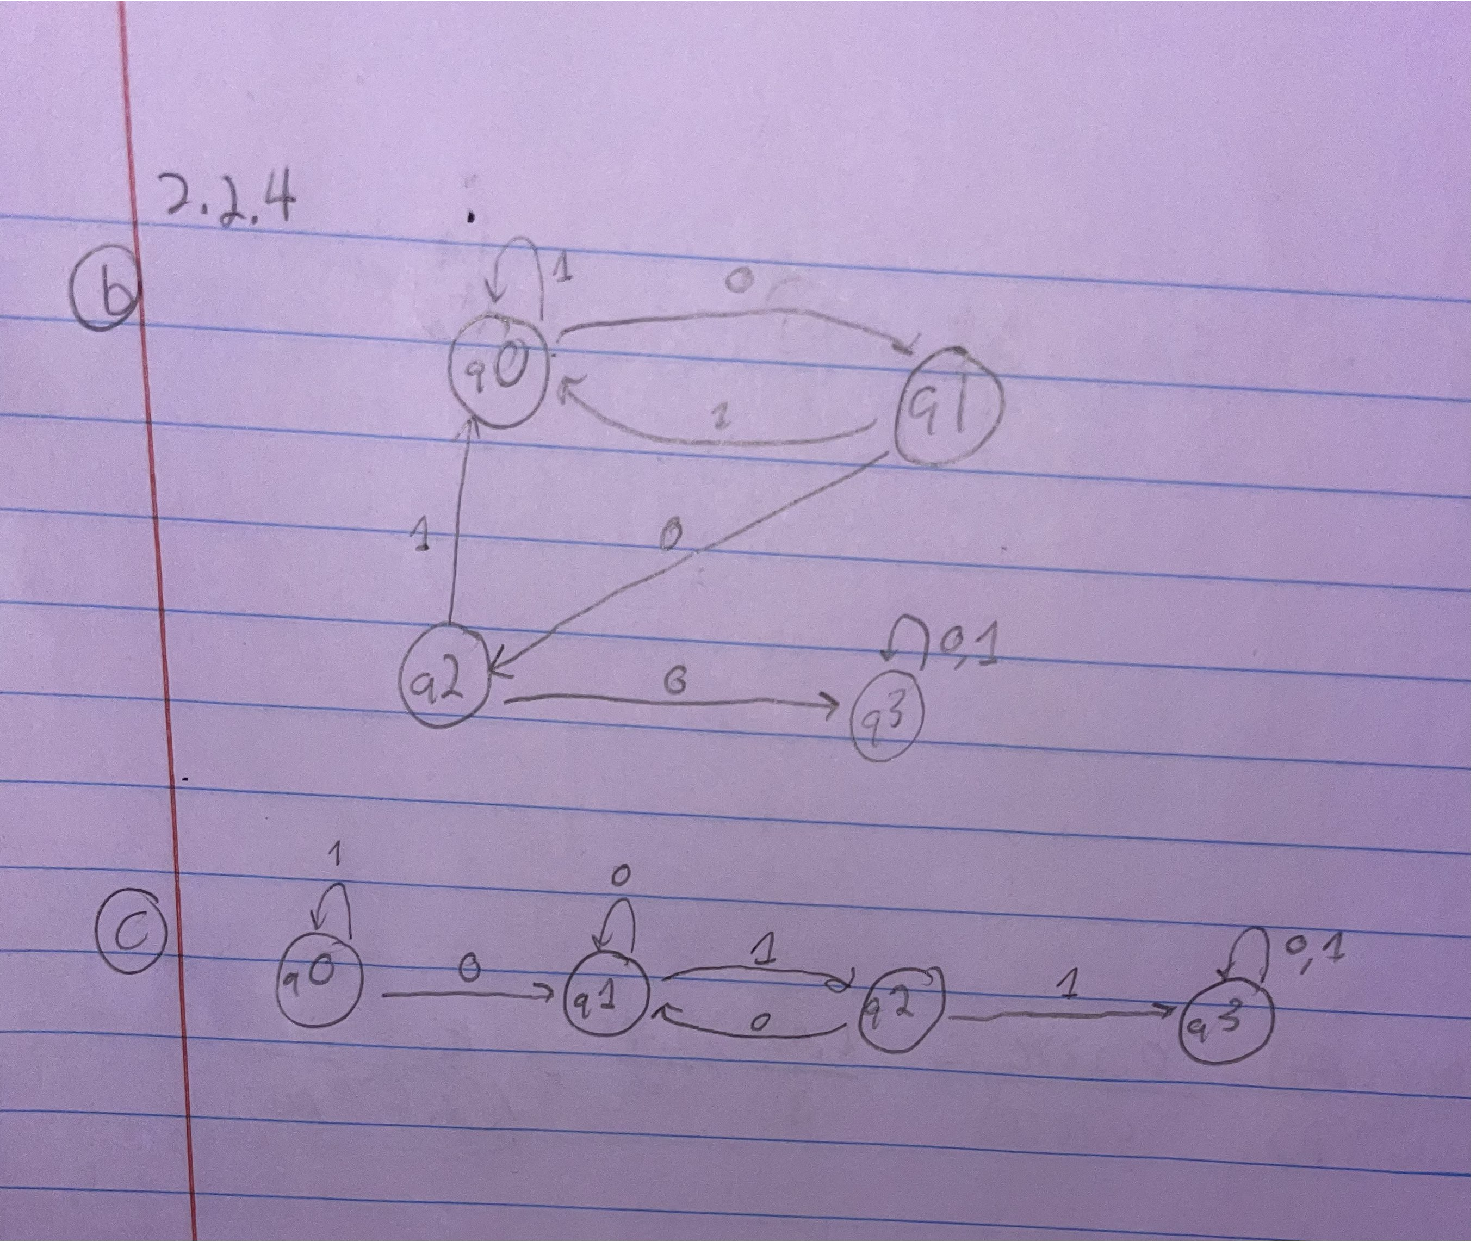
\includegraphics[width=15cm, height=17.5cm]{Week1.pdf}
\end{center}

\subsection{Week 2}

\medskip\begin{center}
\includegraphics[width=15cm, height=20cm]{Week2 (2).pdf}
\end{center}
\clearpage

\subsection{Week 3}
Converting NFAs to DFAs by Hand
\medskip\begin{center}
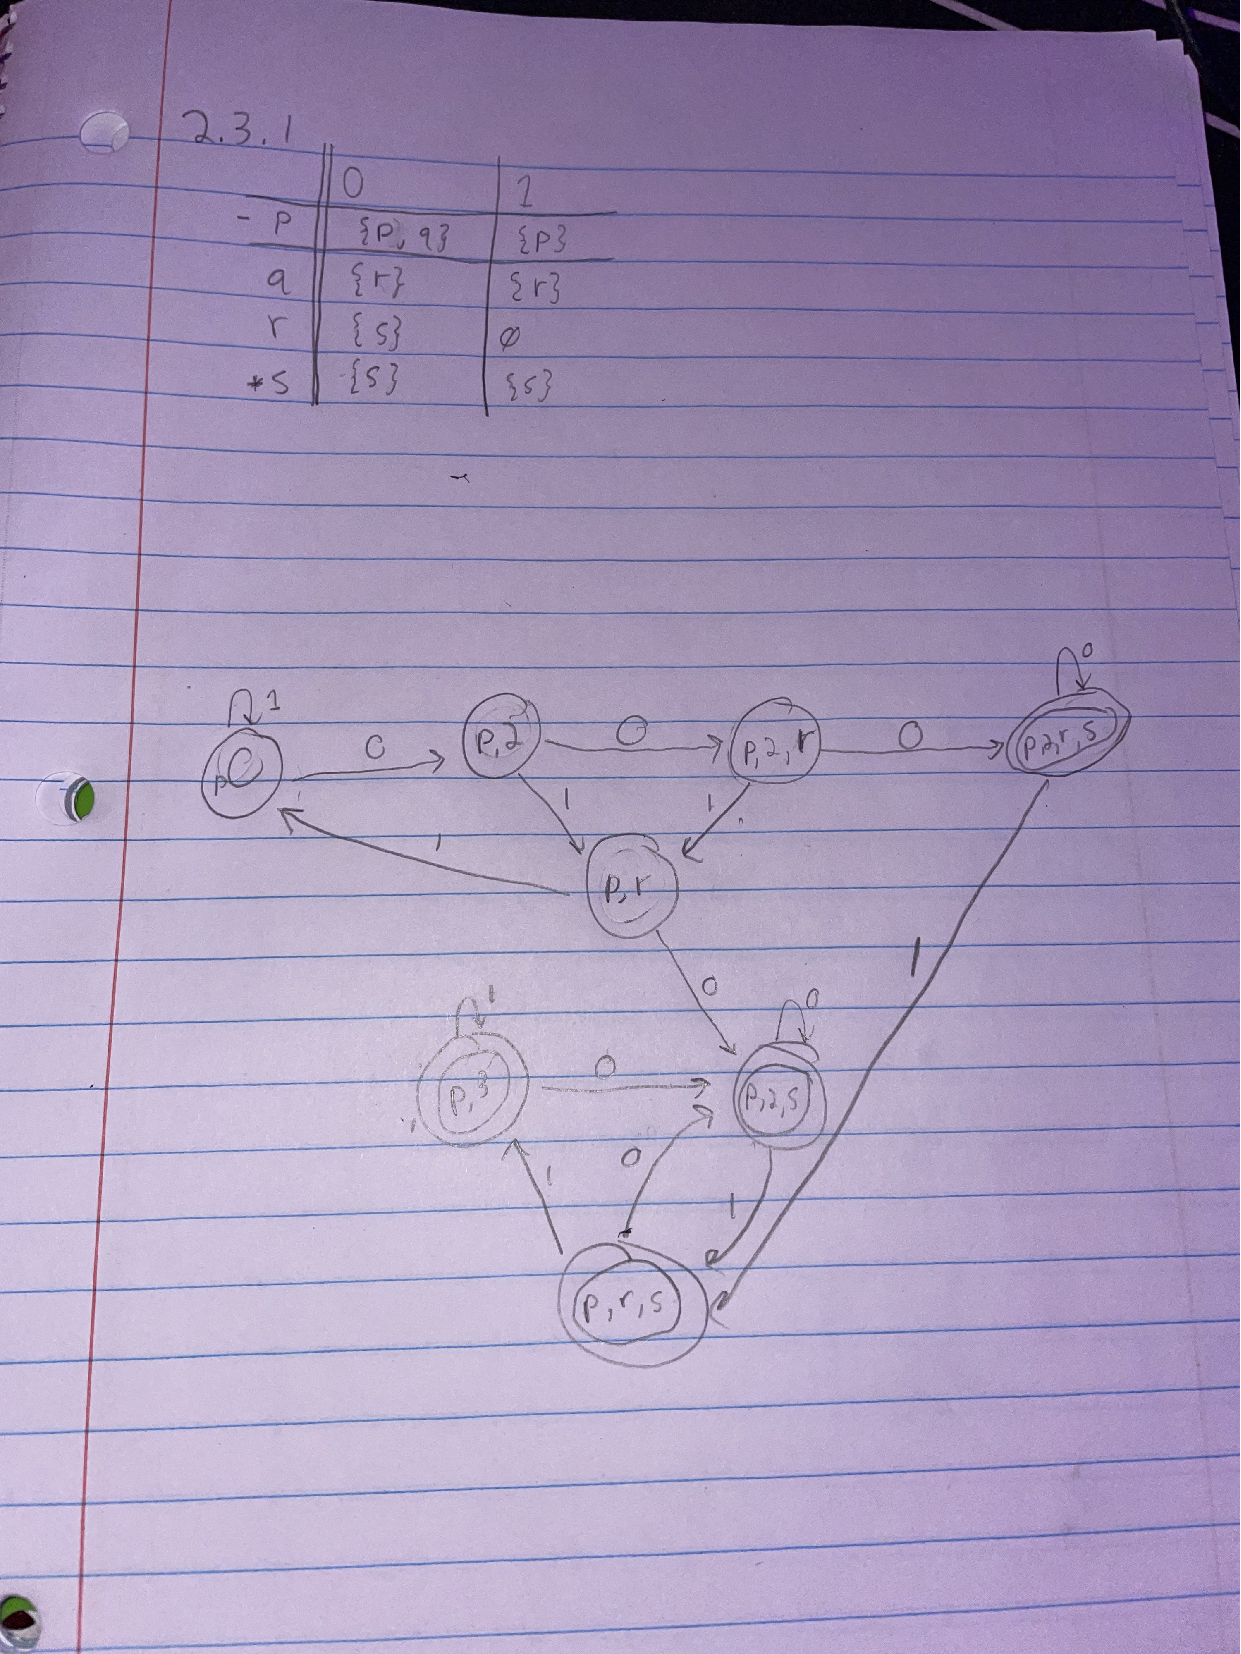
\includegraphics[width=15cm, height=20cm]{Week3.pdf}
\end{center}
\clearpage

Converting NFAs to DFAs In Haskell Using the List Monad
\medskip\begin{center}
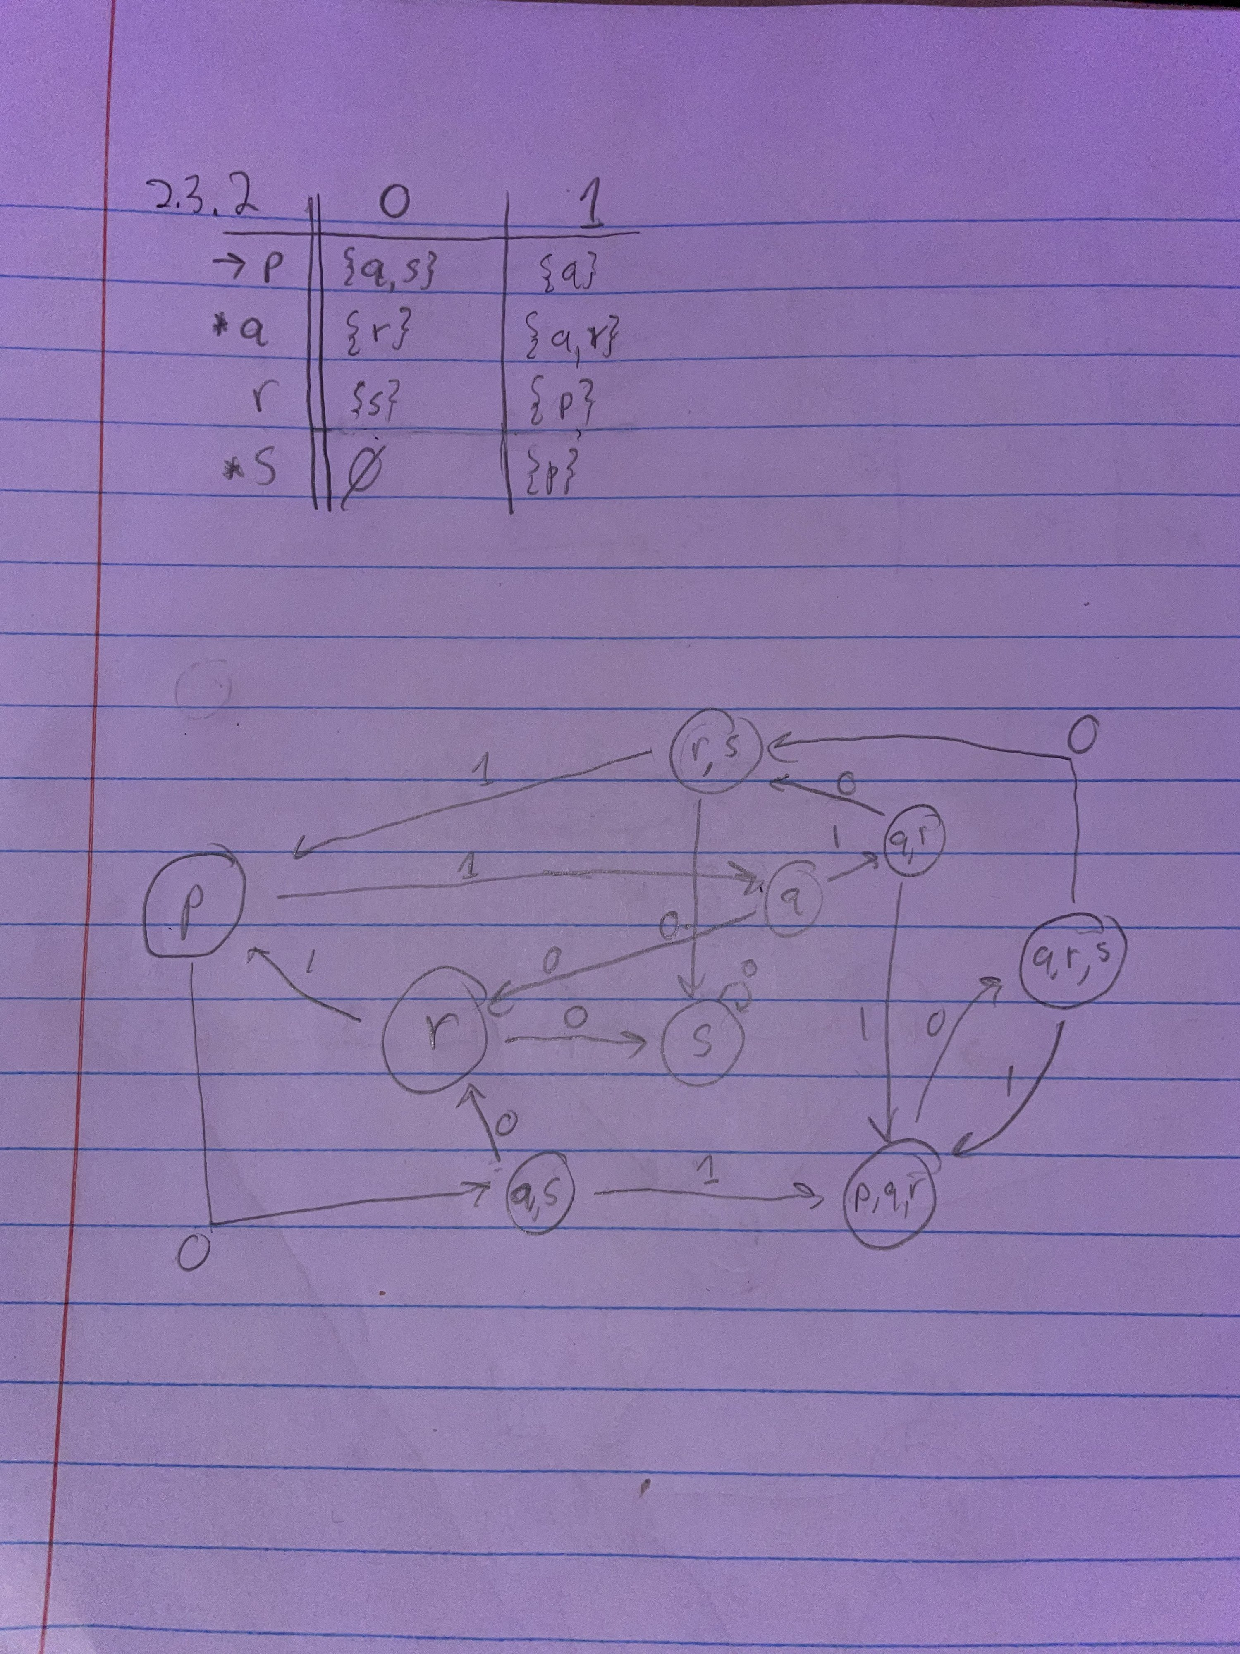
\includegraphics[width=15cm, height=20cm]{Week3P2.pdf}
\end{center}
\clearpage

\subsection{Week4}
Write out the concrete syntax tree for the complete Fibonacci program.
\medskip\begin{center}
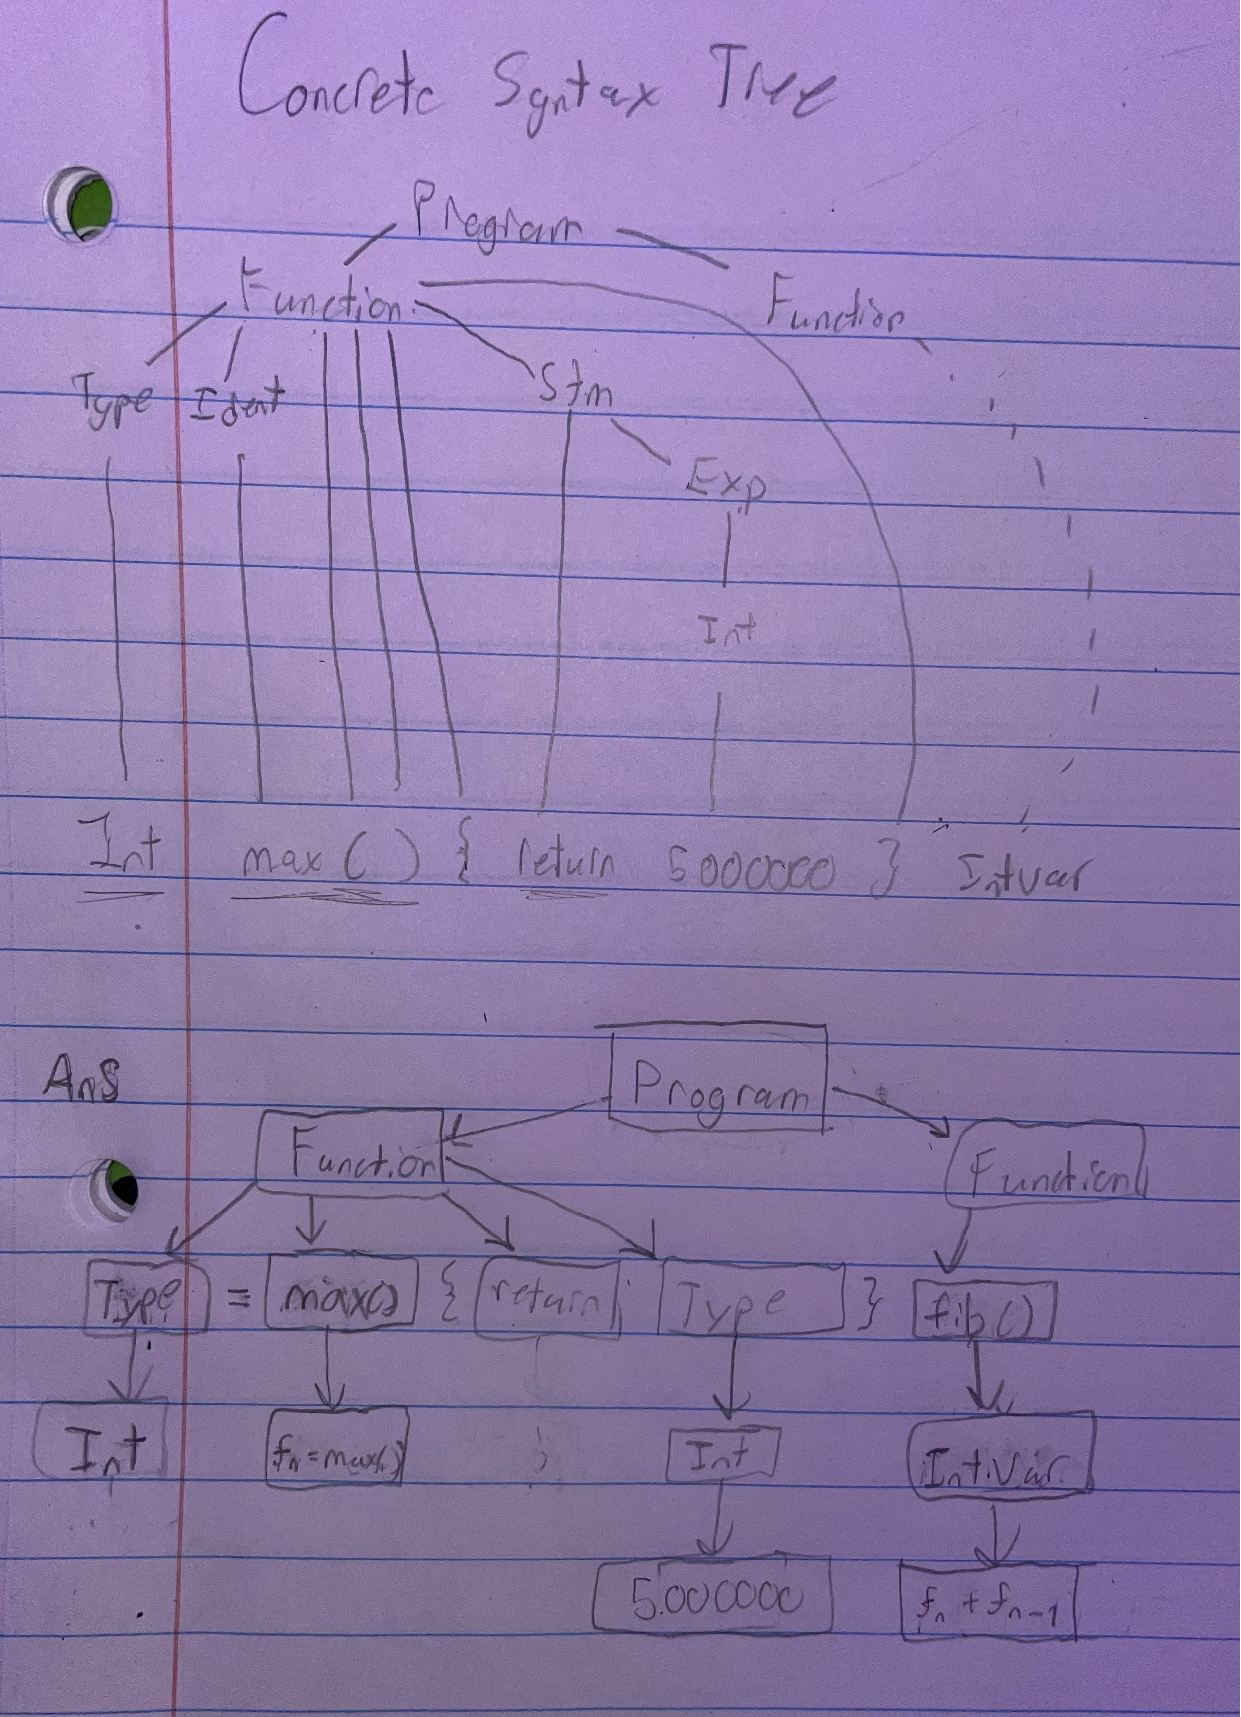
\includegraphics[width=15cm, height=20cm]{Week4P1.pdf}
\end{center}
\clearpage

Write out the abstract syntax tree for the complete Fibonacci program.
\medskip\begin{center}
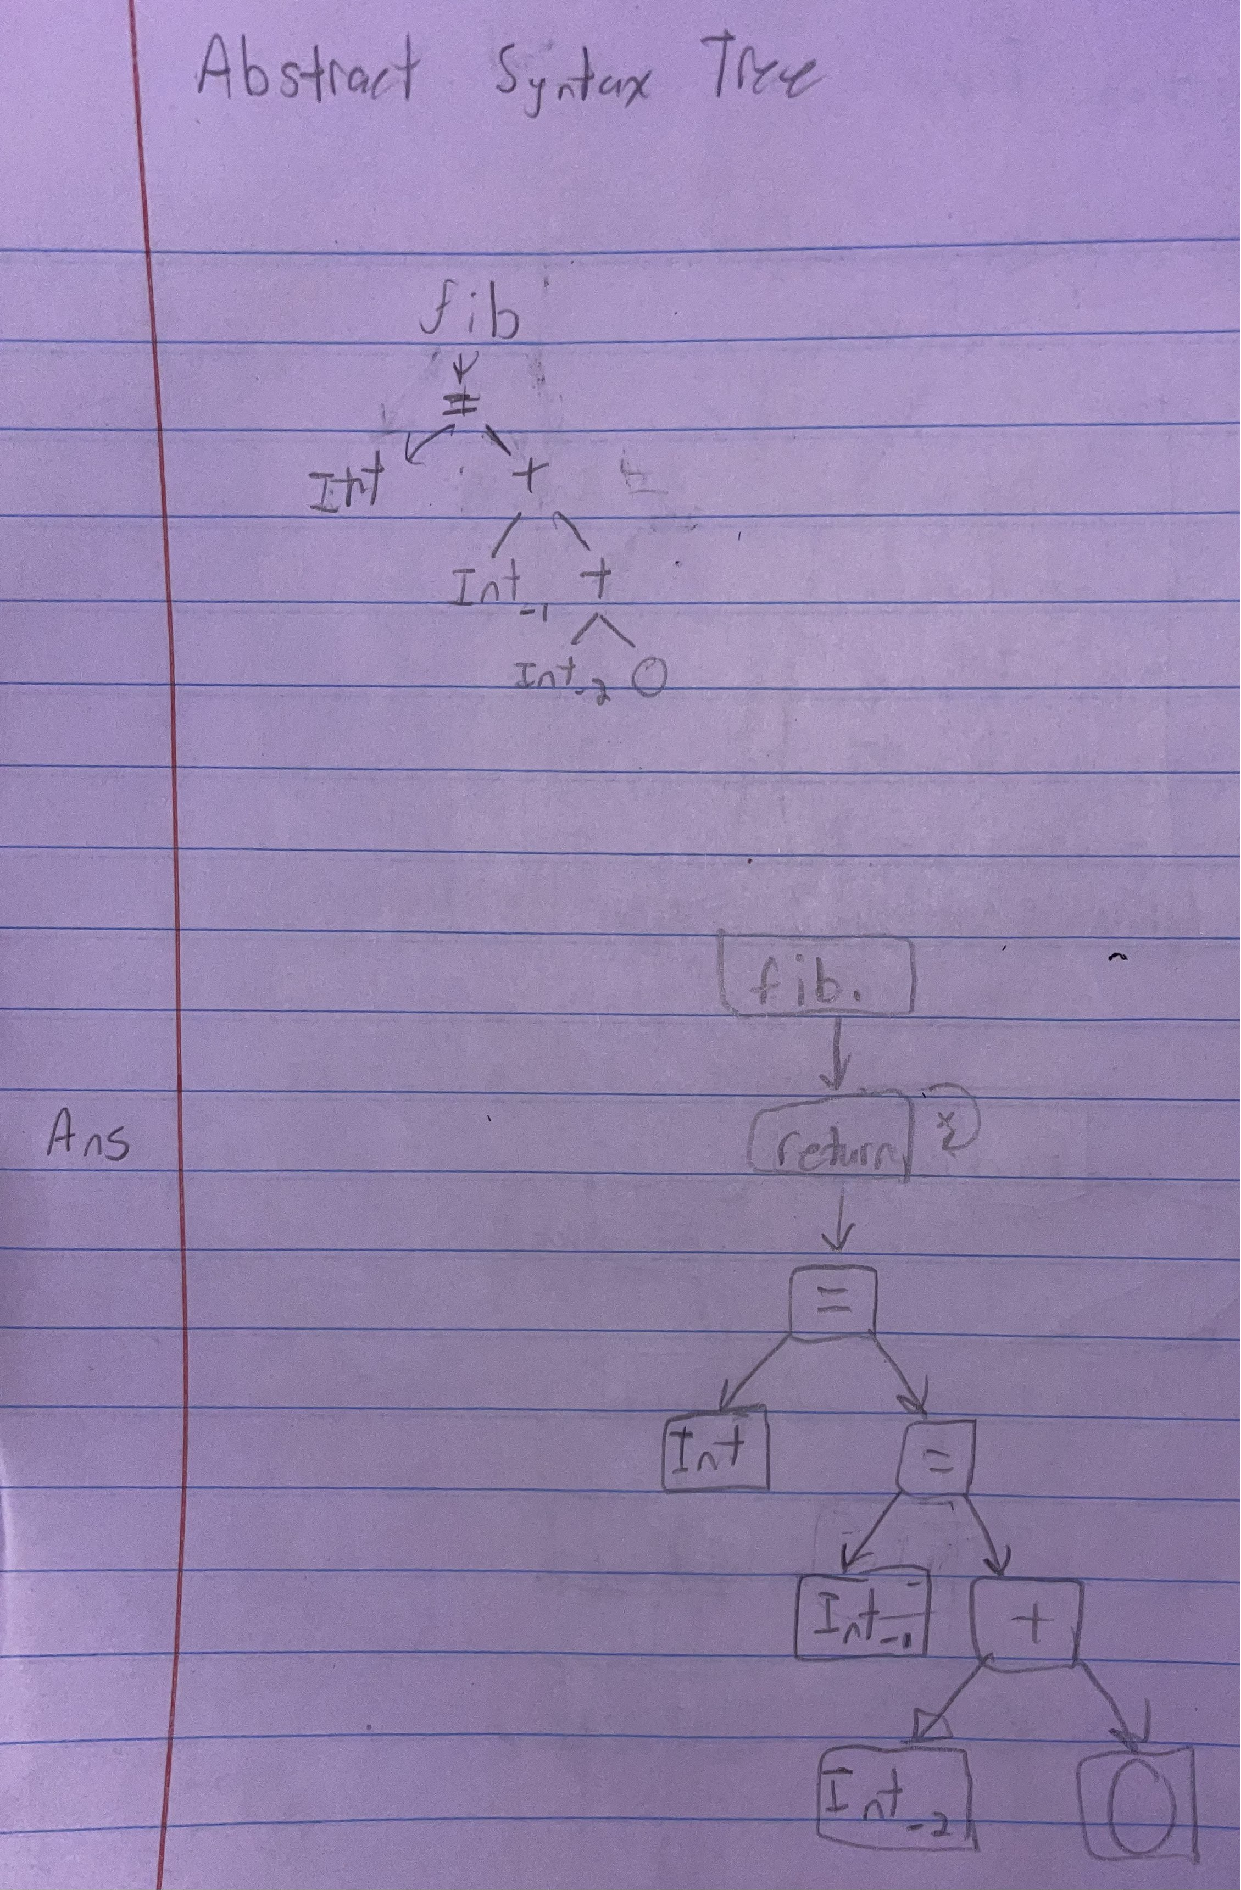
\includegraphics[width=15cm, height=20cm]{Week4P2.pdf}
\end{center}
\clearpage

\subsection{Week10}
Show, in the form of a proof tree, the steps taken by an interpreter evaluating the following program fragment.
\medskip\begin{center}
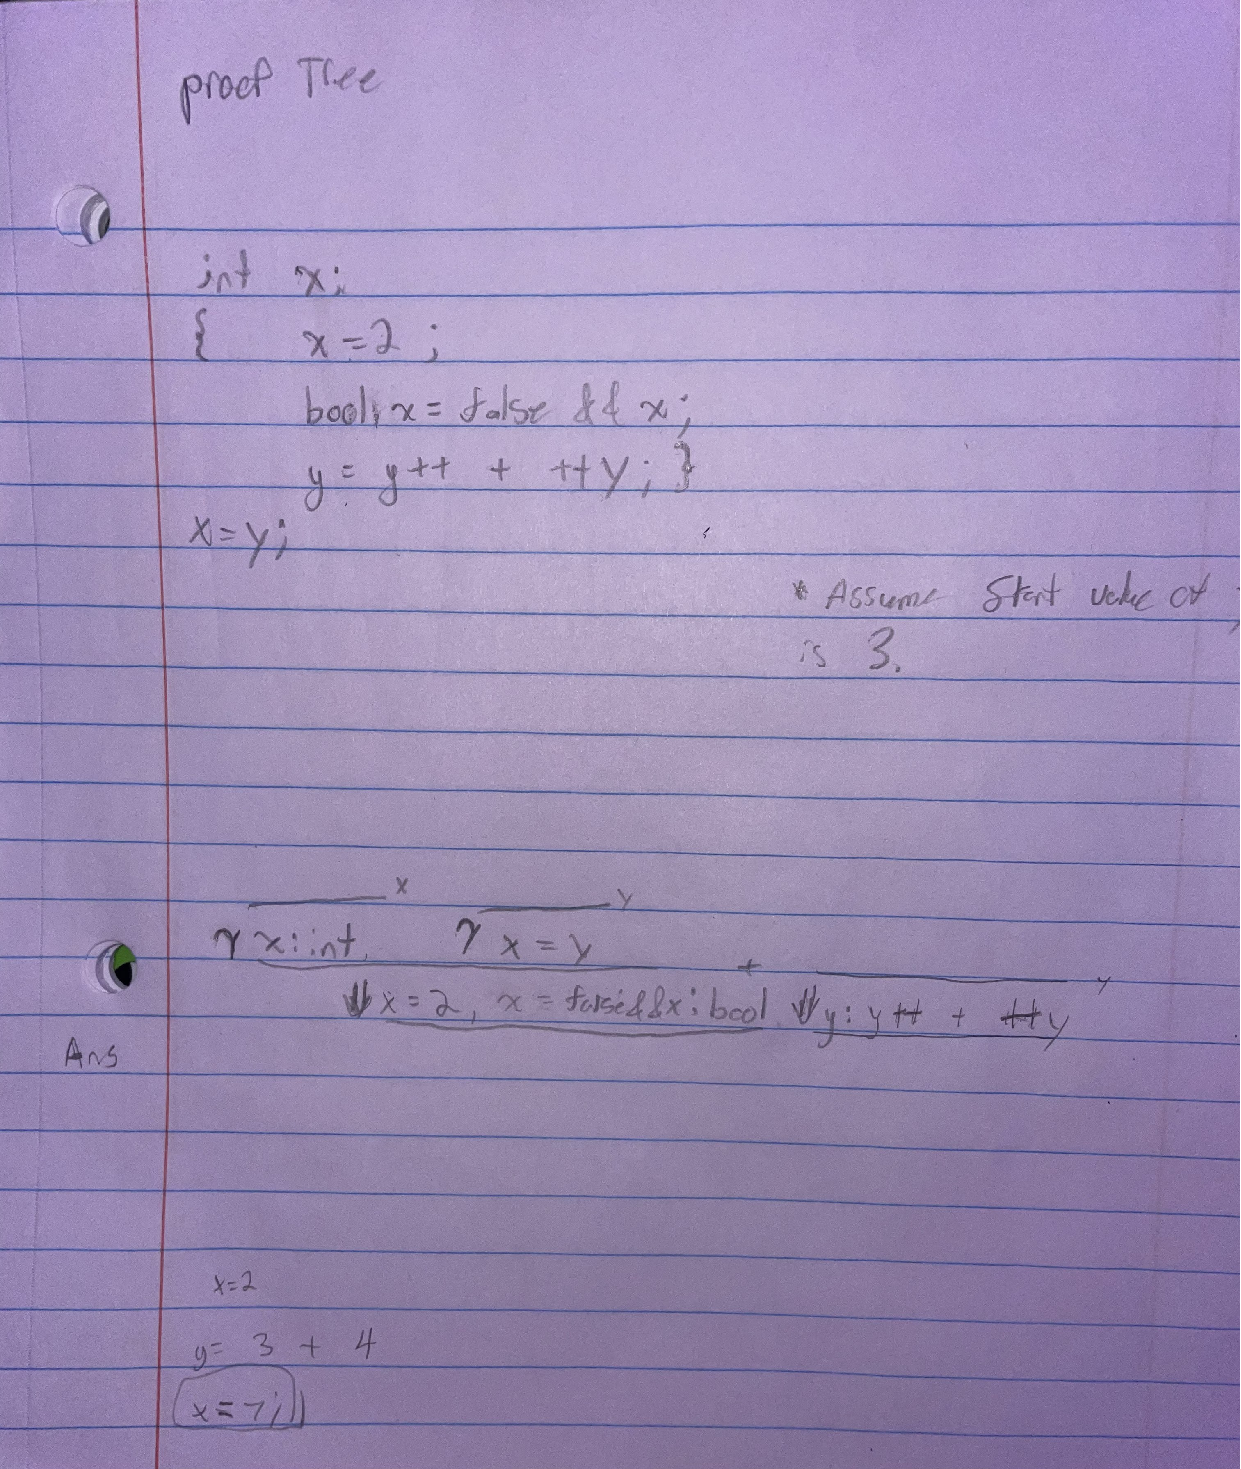
\includegraphics[width=15cm, height=20cm]{Week10.pdf}
\end{center}
\clearpage

\section{Project}
For my research on a compiled programming language, I decided to choose a language and program I am very familiar and comfortable with. C++ was the first new language I learned when attending Chapman. Having already learned Java and Python, the jump to learning C++ was not too difficult to grasp and has become one of my favorites to code in. Additionally, having a game development minor pushed me into explaining how a compiler works with a game due to the extensive work I have done on video games in my past. I am sure everyone at some point in their life has played the game of Tic-Tac-Toe. The rules are pretty straightforward, the first player to connect three of their shapes (X's or O's) either vertically, horizontally, or diagonally wins the game. Another way for the game to end is in a tie. In the case this takes place, a simple bool will be able to determine when a winner is present and when a tie occurs. The board is even easier to set up, consisting of two pairs of parallel lines being perpendicular to each other. Seeing as we have landed on a universally understood game, and a programming language that I have a good amount of experience in, it is now time to dive into how we go from programming in C/C++ to how the machine translates the code into a language it can understand.

Writing code in an interpreter is not the end-all of making a program run and display graphics to the user. Many steps are taken behind the scenes to reduce run-time and compile time. The computer can not understand the plain English and source code that us programmers write in. To accomplish a translation into machine language, or assembly language, the programmer must compile the program with the command "g++ file.cpp". The compiler will check for any syntax or run-time errors before fully compiling. If the code is free of bugs/issues then the compiler will create a file in assembly that significantly reduces the source code. 

The Tic-Tac-Toe program I decided to utilize for visual help was taken from this GitHub repository \href{https://github.com/ssiddique-info/tic-tac-toe-in-c-}{[TTT]} Some changes had to take place because the code would not compile after cloning it to my device. After tweaking some aspects of the code, changing some functions, and adding some supporting header files, it was time to see if compiling would work.

First you open your project folder in the IDE of your choice. I used Atom and used screen captures to display my outputs. After changing directories in the terminal and arriving at the folder you can begin to test the compiler. An example of how compiling looks in the terminal is listed below:

\medskip\begin{center}
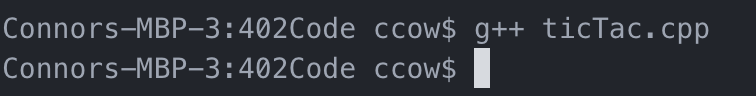
\includegraphics[width=16cm, height=3cm]{Pic1.png}
\end{center}

This is a pretty straightforward step for experienced programmers. However, even some of those who have learned complex programming languages and abstract mathematics do not fully grasp the process of turning a program into assembly language. I have spent a decent portion of my time here at Chapman utilizing C++ for many of my courses. 

A successful compile will return nothing in the terminal and a new file will be added to the project folder you are working in. As mentioned earlier, assembly language is meant to be read and interpreted only by the computer. The new assembly language is then used by the computer to execute the code, after another input is put through (./a.out). It is successful by repeatedly reading the instructions outlined initially and then executing them over and over again through recursion. At first glance, all of the characters in the assembly file look like a bunch of randomized words in no particular order to the average person or programmer. However, that does not mean it is completely impossible to decipher. Let’s take a look at what this would look like when a successful compile occurs:

\medskip\begin{center}
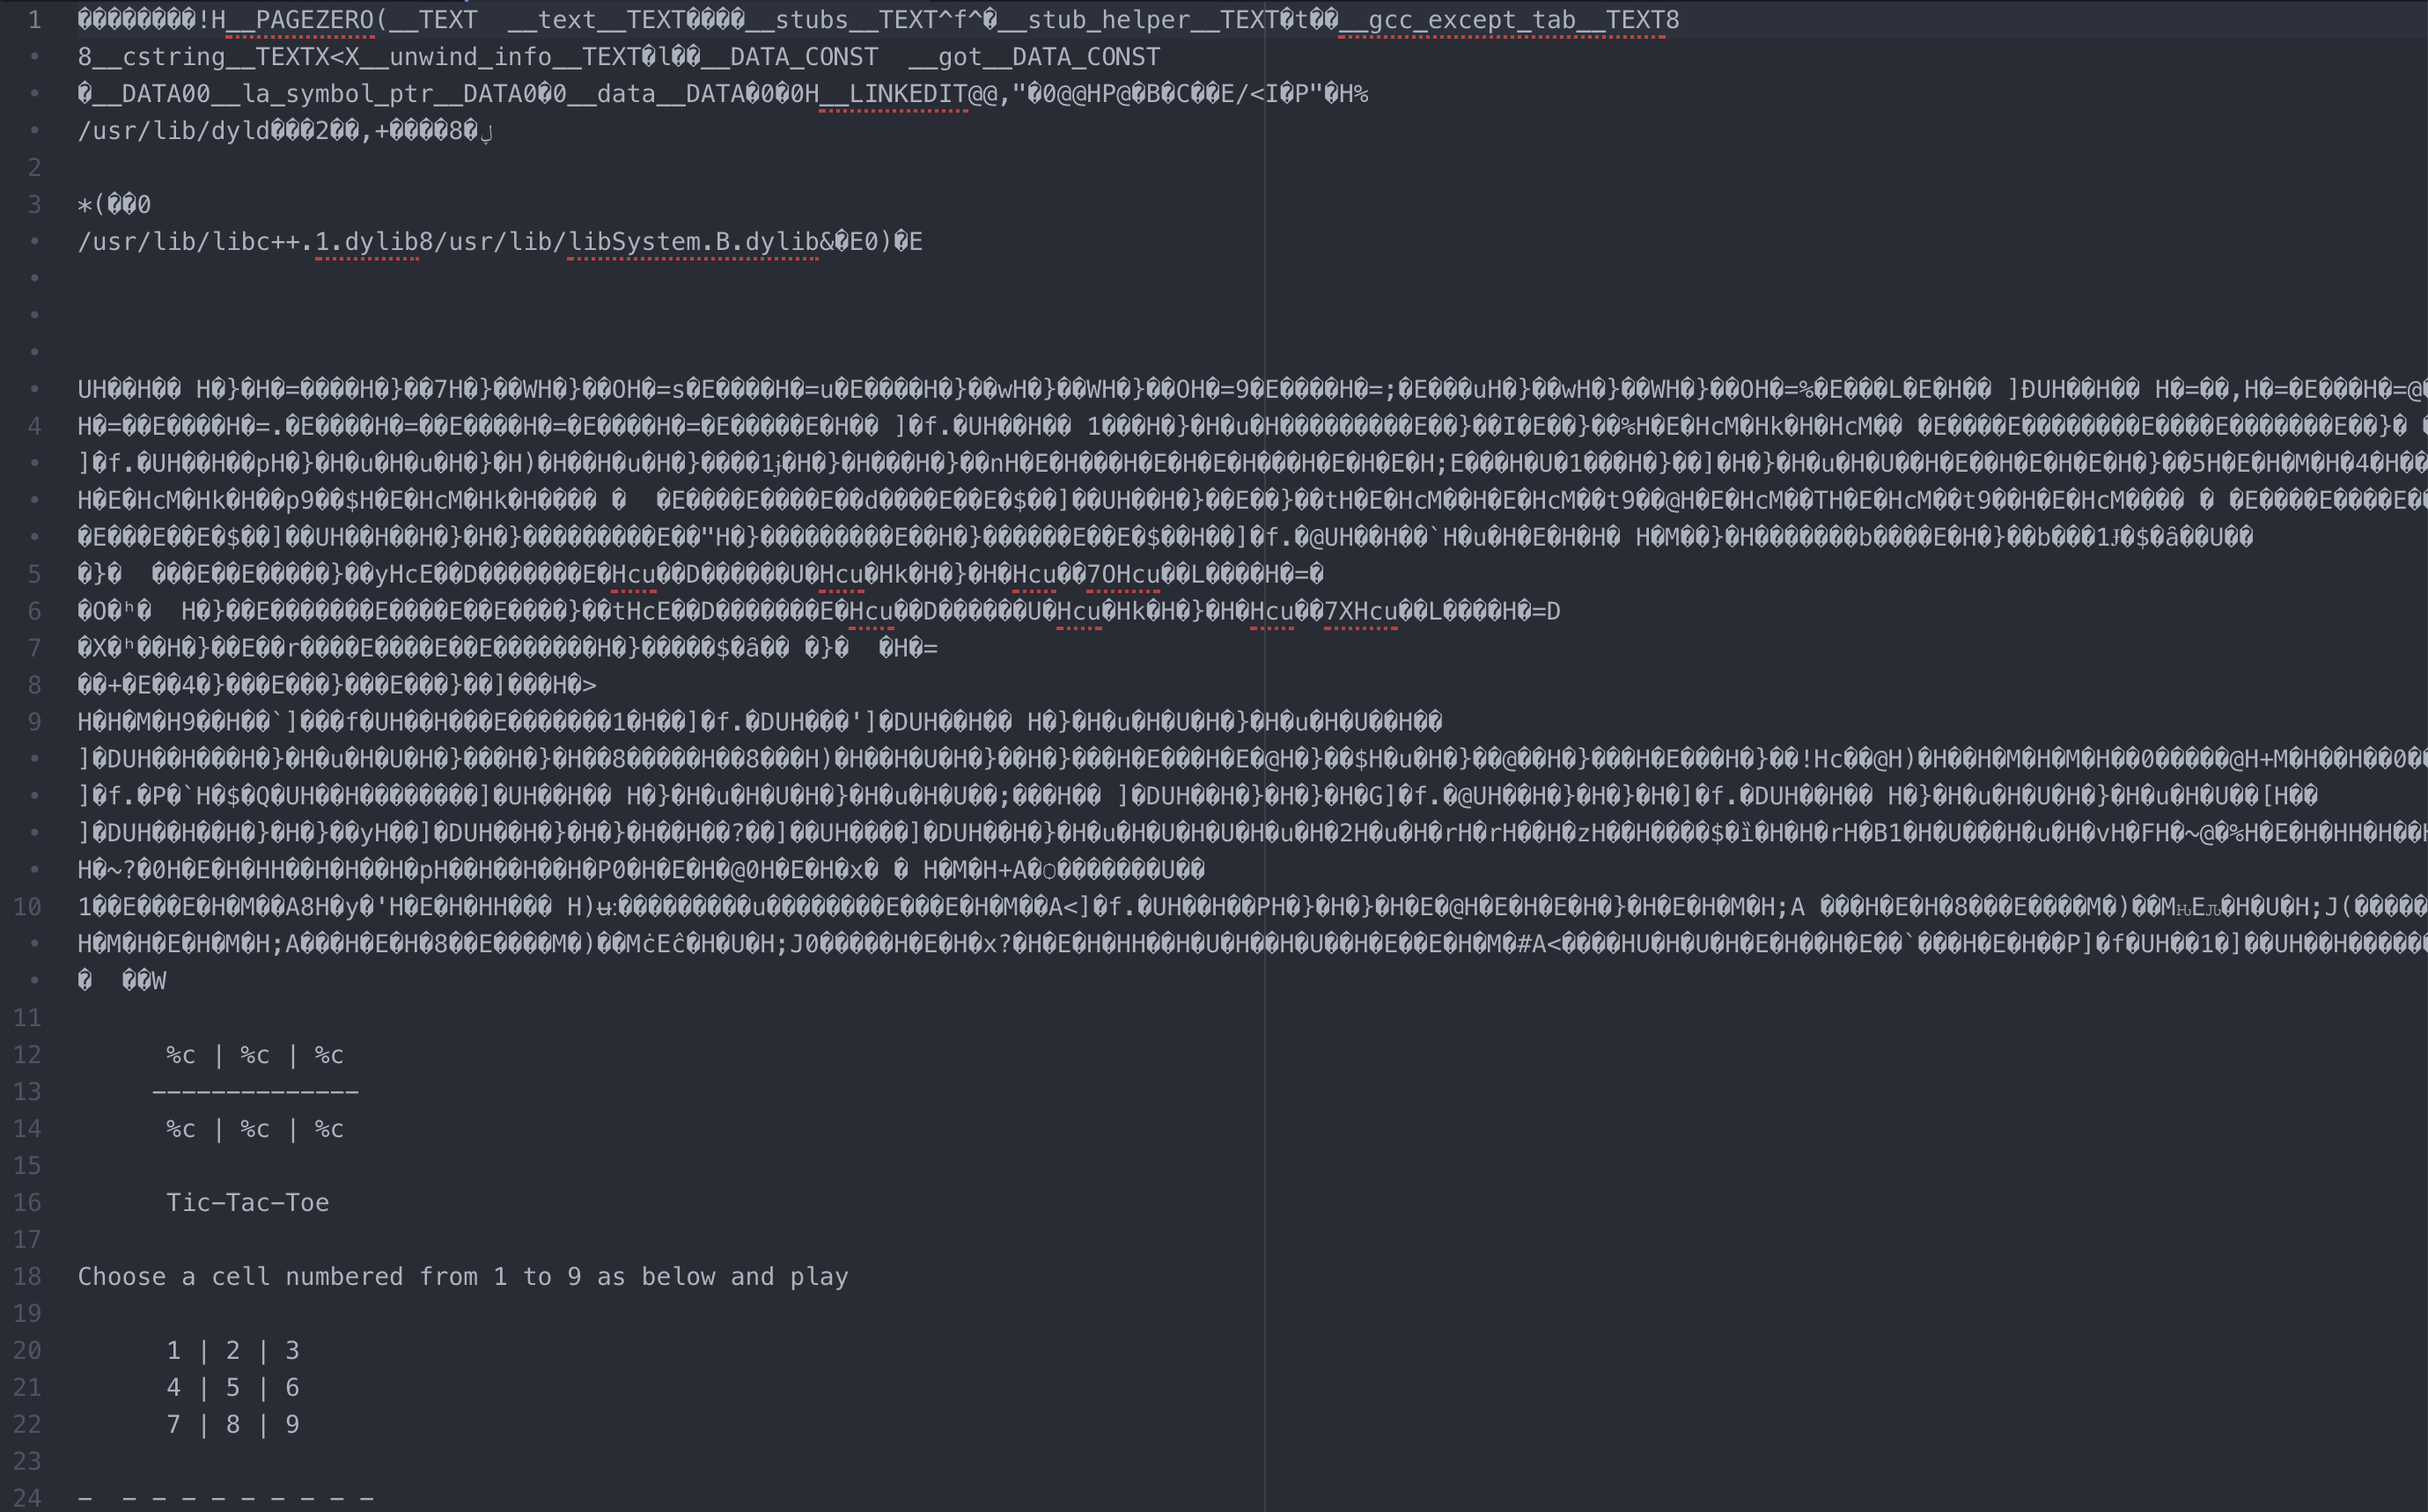
\includegraphics[width=16cm, height=8cm]{Pic2.png}
\end{center}

The compiler creates a new file in the folder you are working in that is designed to be accessed and read by the computer. In Linux, the compiler will create this file named "a.out", an abbreviation for assembly output when no specific file extension is specified. Viewing this file for your own eyes will require you to open it in an IDE or text editor as done in the above example. 

Obviously, this looks like a randomized collection of characters in a file but if we dissect the output we can learn a  bit. The first thing to note is the a.out file is mainly constructed of hexadecimal values. These are the characters that are not in "English" nor integer values. The reason they are not presented in an easy-to-read format is that Atom, the IDE I primarily use, is not equipped to display these characters. An outside library or installation is required to properly display these characters for us to see. However there are some characters that we can interpret and understand from the assembly language. Some of the code that was written in the original .cpp file is still present in this form. More of the a.out file is present below to see these English words:

\medskip\begin{center}
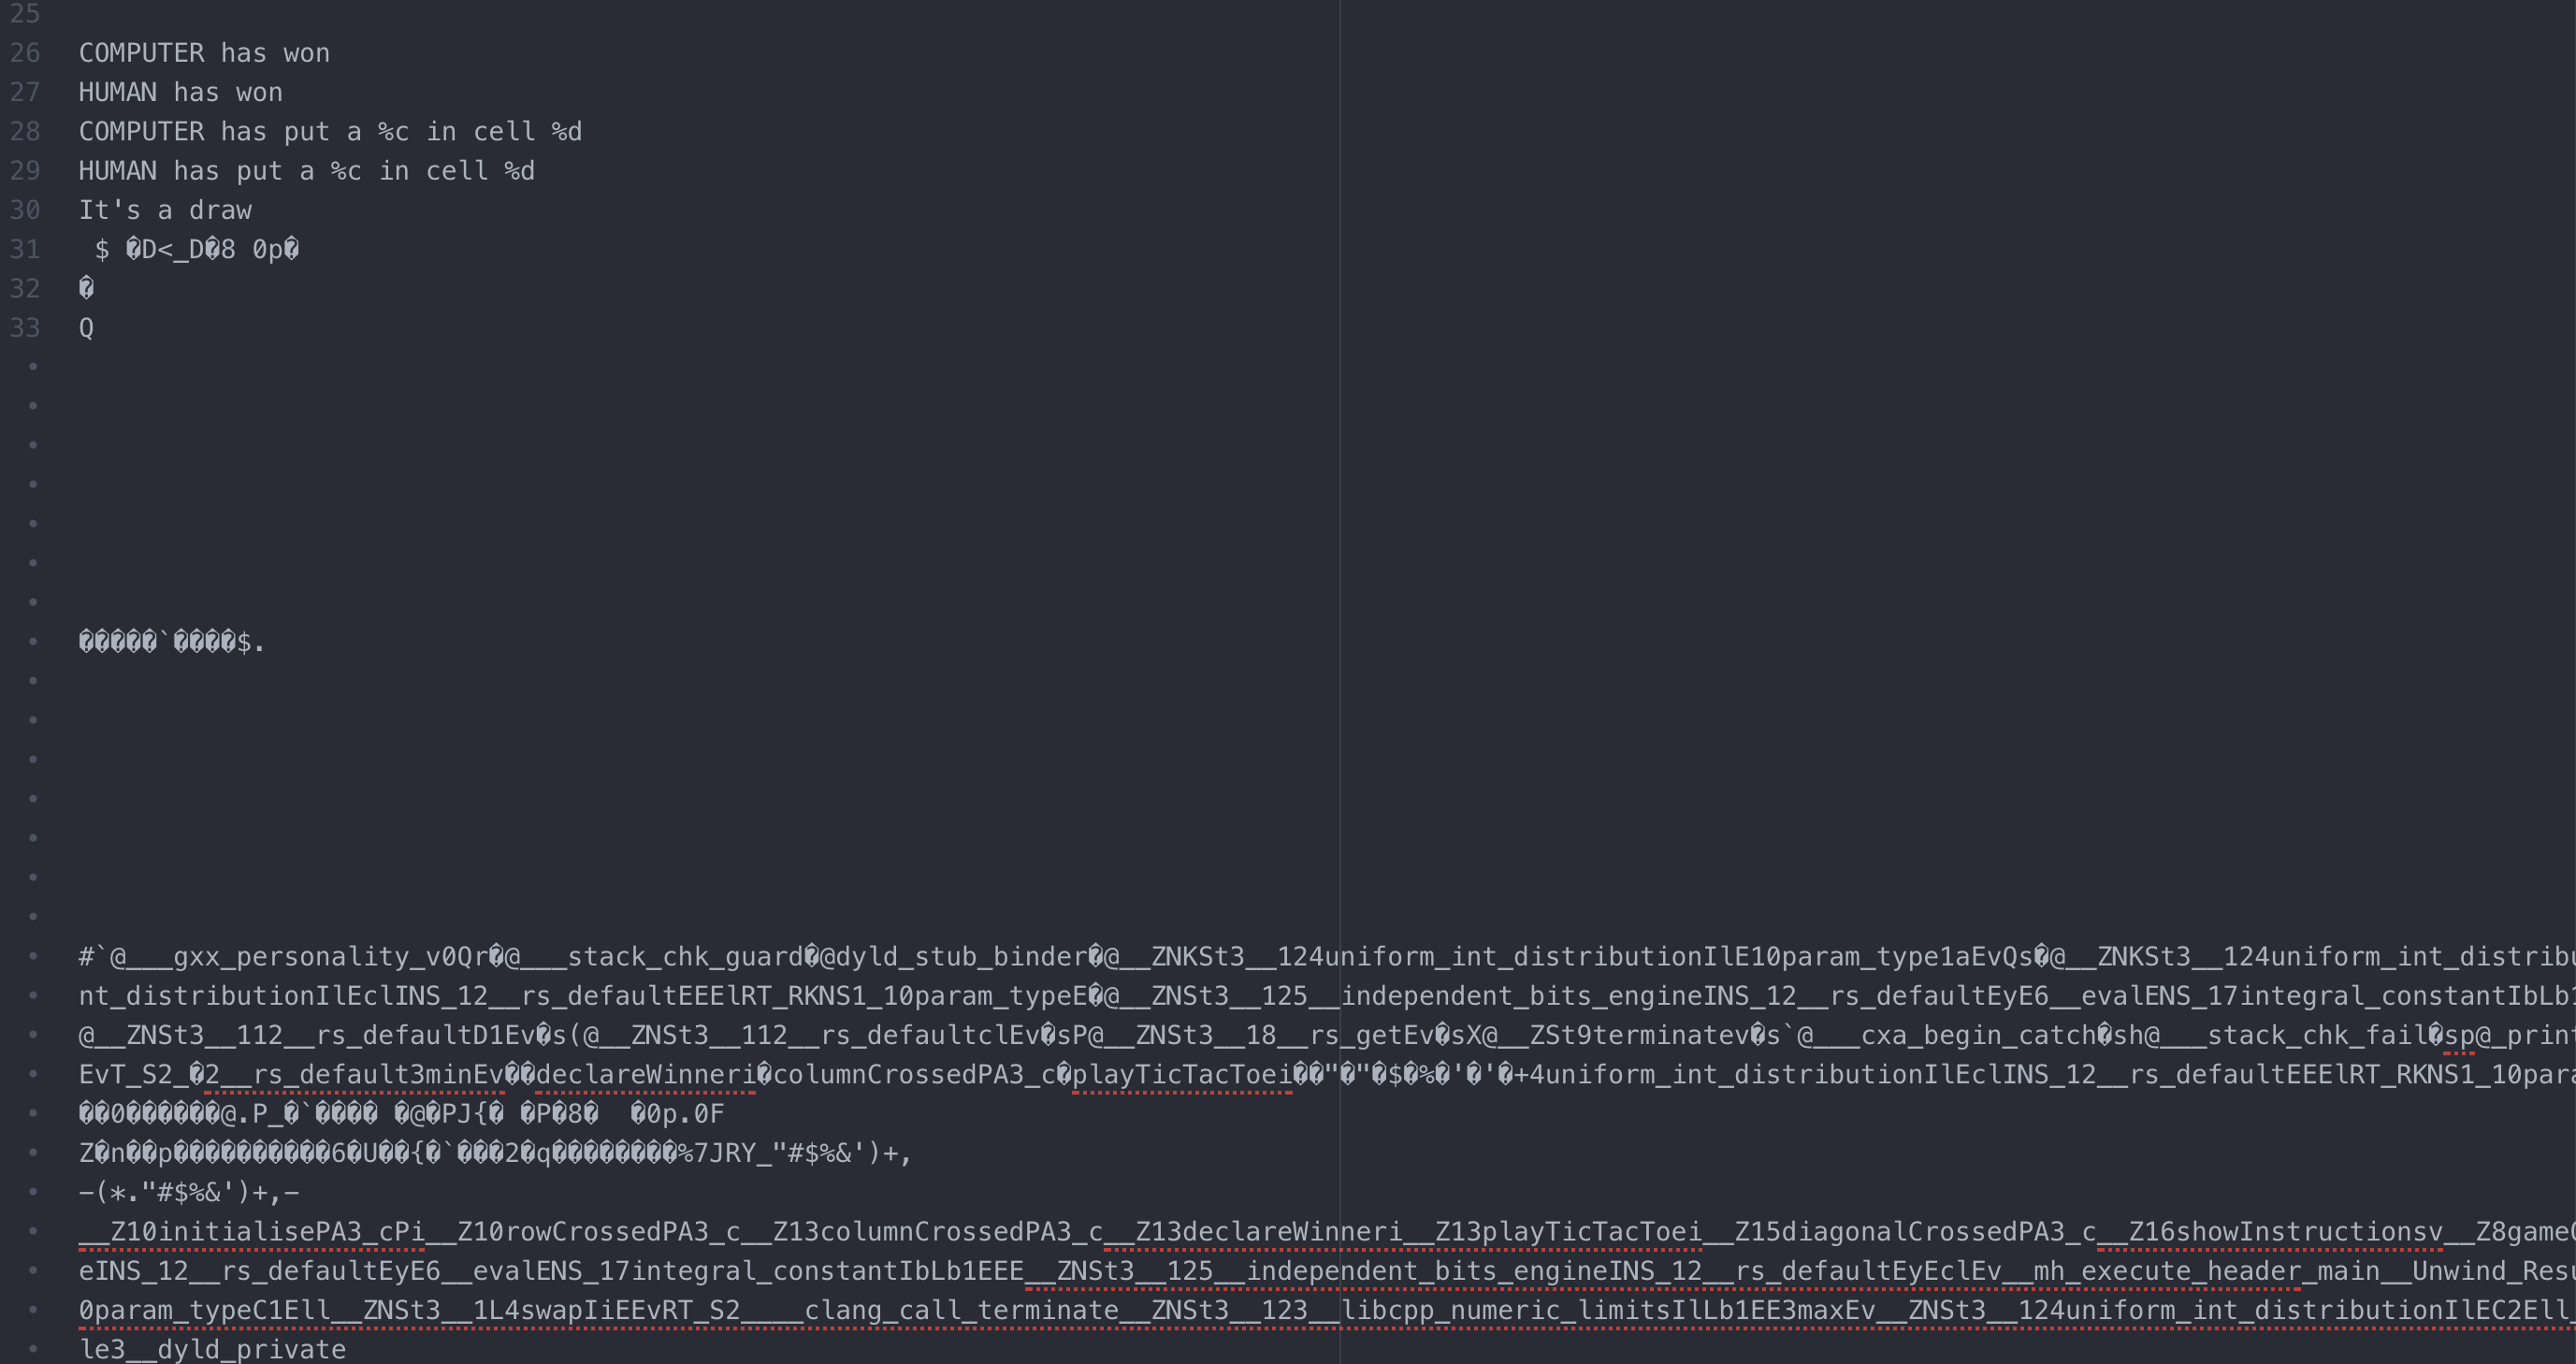
\includegraphics[width=16cm, height=8cm]{Pic3.png}
\end{center}

Line 26 in the a.out file is taken directly from the .cpp file and not altered at all. These easy to read lines are print statements in the C++ file. Additionally some lines have been shortened and changed slightly for run time optimization. Remember this is the standard output when compiling in C++. That means there are different techniques to alter the assembly language when compiling. A simple altering of the terminal input can do massive changes in how we can view this file. Instead of typing "g++ ticTac.cpp" we can add the '-S' flag after g++ (new input: g++ -S ticTac.cpp)\href{https://www.geeksforgeeks.org/compiling-with-g-plus-plus/}{[COM]}. This addition will create a more easy to understand assembly file that us humans can actually interpret.

Another thing to note is the assembly language created from the compiler is a lot denser and shorter than the program written to execute. For example the Tic-Tac-Toe C++ file is 242 after revisions. The a.out file is technically only 33 lines and meant to be read as quickly as possible by the machine. The assembly language is incredibly difficult to learn, near impossible to master, and would require the programmer to spend massive amounts of time learning all the intricacies of the assembly language. Also, programming languages were created to make the translation between English and machine interpreting seamless. Programmers can put their thoughts and ideas into variables and functions with naming conventions that make sense to whoever is writing. After the blueprint is completed then the compiler is called upon to optimize the program and to create as little run-time processing as possible. The assembly language and programming language work in tandem to reduce the final run-time of the program while making coherent sense to the author.

\section{Conclusion}\label{conclusion}

This course has expanded upon the concept of compilers and how the complex mind of a computer works. When I started programming all the way back in high school I was taught how to code "Hello World" like every other programmer starting their journey. However the underlying aspects of how does this or that work were never an important topic of conversation. That has since changed when I took Programming Languages last semester. There are a vast amount of languages that are better suited for various tasks. Learning what each and every language is strong at is vital for cutting down on mistakes and optimizing a program for a business, science experiment, etc. The introduction of Haskell was a shocking topic to wrap my head around. For years I had thought most video games, operating systems, car computers, etc. were just variations of languages like Java, C/C++, or Python. Thankfully I have a better understanding of how a computer works on a software level, and how different commands can access various parts of the hardware. The grammar aspect of this course was definitely similar in some ways to last semester, however I found myself stuck on numerous occasions looking up how to add two integers. Mastery of any skill comes with time and practice. The lessons learned in this course will stay with me throughout my career in the computer science field. Although Haskell is not widely used as it was in the past, having the various knowledge of other languages is much more beneficial than being proficient in a single one like Python. Although I never fully created my own language from scratch, I can appreciate how much time and effort goes into constructing such a complex interface. One of the biggest takeaways from this course is the fact that there are countless possibilities to the things us programmers can create. We are limited in the capacity of our imagination. The fact that we have gone from functional programming languages like Haskell and simplified the idea into compiled languages like Java means we can go even further to make programming accessible and available for everyone to use. Some people are immediately turned off to the idea because it looks too difficult to learn. As technology continuously advances, we must stay up to date and continue to make things easier to utilize. One fact that always reminds me of where we are heading, scientifically, is that it only took 4KB of RAM to land the Apollo 11 on the moon. Meanwhile the iPhone 13 has 6GB of memory, meaning the device you use everyday is a lot more powerful than the computer that landed men on another planet. Everyday we, as society, are only getting smarter and finding new ways to make our lives easier. Programming is the front line of the advancement and this course has opened my eyes to what possibilities exist and what boundaries will be toppled.

\begin{thebibliography}{99}
\bibitem[HMU]{Hopcroft}
	John E. Hopcroft, Rajeev Motwani, Jeffrey D. Ullman:
\href{http://ce.sharif.edu/courses/94-95/1/ce414-2/resources/root/Text%20Books/Automata/John%20E.%20Hopcroft,%20Rajeev%20Motwani,%20Jeffrey%20D.%20Ullman-Introduction%20to%20Automata%20Theory,%20Languages,%20and%20Computations-Prentice%20Hall%20(2006).pdf}{Introduction to automata theory, languages, and computation,} 3rd Edition. Pearson international edition, Addison-Wesley 2007
\bibitem[TTT]{Tic-Tac-Toe in C++}
    Developer Resources:
\href{https://github.com/ssiddique-info/tic-tac-toe-in-c-/}{Tic Tac Toe GitHub}
\bibitem[COM]{Compiling with g++}
    GeeksforGeeks:
\href{https://www.geeksforgeeks.org/compiling-with-g-plus-plus/}{Compile with g++}

\end{thebibliography}

\end{document}